% !TeX program = pdflatex
\documentclass[10pt,a4paper,landscape]{article}
\usepackage[a4paper,landscape,margin=9mm]{geometry}
\usepackage[T1]{fontenc}
\usepackage[utf8]{inputenc}
\usepackage{tgheros}
\renewcommand*\familydefault{\sfdefault}
\usepackage{microtype}
\usepackage{xcolor}
\usepackage{array}
\usepackage{booktabs}
\usepackage{adjustbox}
\usepackage{tikz}
\usetikzlibrary{arrows.meta}
\pagestyle{empty}
\setlength{\parindent}{0pt}
\definecolor{ink}{RGB}{25,35,55}
\definecolor{surface}{RGB}{245,248,252}
\definecolor{primary}{RGB}{0,82,155}
\definecolor{profit}{RGB}{21,122,78}
\definecolor{profitbg}{RGB}{220,245,230}
\definecolor{warnstroke}{RGB}{197,48,48}
\definecolor{routeb}{RGB}{88,55,160}
\newcommand{\statlabel}[1]{{\fontsize{6.5}{8}\selectfont\bfseries\textls[120]{\textcolor{ink!55}{\MakeUppercase{#1}}}}}
\newcommand{\bridgebadge}[2]{\tikz[baseline=(b.base)]{\node[draw=#2,fill=#2!10,rounded corners=1mm,inner xsep=1.6mm,inner ysep=0.5mm](b){{\fontsize{6.6}{8}\selectfont\bfseries\textcolor{#2}{#1}}};}}
\newcommand{\stepnum}[1]{\tikz[baseline=(s.base)]{\node[circle,fill=primary,inner sep=0.5mm,minimum size=3.3mm](s){{\fontsize{5.8}{6.2}\selectfont\bfseries\color{white}#1}};}}
\begin{document}
\color{ink}
{\fontsize{16}{18}\selectfont\bfseries\color{primary} VCHF Menace --- Loop Routes}~{\fontsize{10}{12}\selectfont\textcolor{ink!55}{(VCHF)}}\\[1pt]
{\fontsize{8.5}{10.5}\selectfont Platform-first treasury · same-asset round trips · VCHF held on VNX · chains hold hub stables only}\\[1pt]
{\fontsize{6.8}{8.2}\selectfont\textcolor{ink!55}{2026-06-20 19:13 UTC · docs/vchf-menace-routes-executive.pdf · generated from src/scanner/routes.active\_loops()}}
\vspace{1.5mm}\noindent\rule{\linewidth}{0.3pt}\vspace{1.5mm}
\noindent\begin{tabular}{@{}>{\centering\arraybackslash}p{0.185\linewidth}>{\centering\arraybackslash}p{0.185\linewidth}>{\centering\arraybackslash}p{0.185\linewidth}>{\centering\arraybackslash}p{0.185\linewidth}>{\centering\arraybackslash}p{0.185\linewidth}@{}}
\fcolorbox{profit!35}{profitbg}{\begin{minipage}[c][11mm][c]{0.9\linewidth}\statlabel{Loops}{\fontsize{11}{13}\selectfont\bfseries\textcolor{profit}{12}}\end{minipage}} &
\fcolorbox{primary!25}{surface}{\begin{minipage}[c][11mm][c]{0.9\linewidth}\statlabel{Loop 1}{\fontsize{10}{12}\selectfont\bfseries 3}\end{minipage}} &
\fcolorbox{primary!25}{surface}{\begin{minipage}[c][11mm][c]{0.9\linewidth}\statlabel{Loop 2}{\fontsize{10}{12}\selectfont\bfseries 3}\end{minipage}} &
\fcolorbox{primary!25}{surface}{\begin{minipage}[c][11mm][c]{0.9\linewidth}\statlabel{Loop 3}{\fontsize{10}{12}\selectfont\bfseries 6}\end{minipage}} &
\fcolorbox{primary!25}{surface}{\begin{minipage}[c][11mm][c]{0.9\linewidth}\statlabel{Bridges}{\fontsize{7}{8.5}\selectfont\bfseries CCTP · Wormhole · ETH 2-hop}\end{minipage}} \\
\end{tabular}
\vspace{1.6mm}\noindent\rule{\linewidth}{0.3pt}\vspace{1.5mm}
\noindent\begin{minipage}[t]{0.46\linewidth}
{\fontsize{9}{11}\selectfont\bfseries\color{primary} Loop families}\\[1.5mm]
\noindent\fcolorbox{primary!35}{primary!6}{\begin{minipage}{\dimexpr\linewidth-2\fboxsep-2\fboxrule\relax}
{\fontsize{8.5}{10}\selectfont\bfseries\color{primary} Loop 1 · Outbound}\\[1.2mm]
{\fontsize{7}{9}\selectfont
\stepnum{1}~Withdraw token: \textbf{platform $\rightarrow$ chain X}\\[0.5mm]
\stepnum{2}~Sell token for stable on chain X\\[0.5mm]
\stepnum{3}~Bridge stable \textbf{X $\rightarrow$ ETH hub}\\[0.5mm]
\stepnum{4}~Deposit USDC \textbf{ETH $\rightarrow$ VNX}\\[0.5mm]
\stepnum{5}~\textbf{Platform buy-back} $\Rightarrow$ same token on platform\\[0.5mm]
}\end{minipage}}
\\[1.4mm]
\noindent\fcolorbox{profit!35}{profit!6}{\begin{minipage}{\dimexpr\linewidth-2\fboxsep-2\fboxrule\relax}
{\fontsize{8.5}{10}\selectfont\bfseries\color{profit} Loop 2 · Inbound}\\[1.2mm]
{\fontsize{7}{9}\selectfont
\stepnum{1}~Platform sell token for USDC\\[0.5mm]
\stepnum{2}~Withdraw USDC \textbf{platform $\rightarrow$ ETH}\\[0.5mm]
\stepnum{3}~Bridge stable \textbf{ETH $\rightarrow$ chain X}\\[0.5mm]
\stepnum{4}~\textbf{On-chain buy-back} token on chain X\\[0.5mm]
\stepnum{5}~Deposit token \textbf{X $\rightarrow$ VNX}\\[0.5mm]
}\end{minipage}}
\\[1.4mm]
\noindent\fcolorbox{routeb!35}{routeb!6}{\begin{minipage}{\dimexpr\linewidth-2\fboxsep-2\fboxrule\relax}
{\fontsize{8.5}{10}\selectfont\bfseries\color{routeb} Loop 3 · Cross}\\[1.2mm]
{\fontsize{7}{9}\selectfont
\stepnum{1}~Withdraw token: \textbf{platform $\rightarrow$ chain A}\\[0.5mm]
\stepnum{2}~Sell token for stable on chain A\\[0.5mm]
\stepnum{3}~\textbf{Direct bridge} stable \textbf{A $\rightarrow$ B} (CCTP preferred)\\[0.5mm]
\stepnum{4}~\textbf{On-chain buy-back} token on chain B\\[0.5mm]
\stepnum{5}~Deposit token \textbf{B $\rightarrow$ VNX}\\[0.5mm]
}\end{minipage}}
\end{minipage}\hfill\begin{minipage}[t]{0.50\linewidth}
{\fontsize{9}{11}\selectfont\bfseries\color{primary} Loops}\\[1.5mm]
{\fontsize{7.4}{9.4}\selectfont\renewcommand{\arraystretch}{1.25}
\adjustbox{max width=\linewidth}{
\begin{tabular}{@{}clll@{}}\toprule
\textbf{\#} & \textbf{Family} & \textbf{Route} & \textbf{Bridge} \\\midrule
1 & Loop 1 · Outbound & Celo & \bridgebadge{Wormhole}{primary} \\
2 & Loop 2 · Inbound & Celo & \bridgebadge{Wormhole}{primary} \\
3 & Loop 1 · Outbound & Base & \bridgebadge{CCTP}{routeb} \\
4 & Loop 2 · Inbound & Base & \bridgebadge{CCTP}{routeb} \\
5 & Loop 1 · Outbound & Solana & \bridgebadge{CCTP}{routeb} \\
6 & Loop 2 · Inbound & Solana & \bridgebadge{CCTP}{routeb} \\
7 & Loop 3 · Cross & Celo $\rightarrow$ Base & \bridgebadge{ETH 2-hop}{warnstroke} \\
8 & Loop 3 · Cross & Celo $\rightarrow$ Solana & \bridgebadge{Wormhole}{primary} \\
9 & Loop 3 · Cross & Base $\rightarrow$ Celo & \bridgebadge{ETH 2-hop}{warnstroke} \\
10 & Loop 3 · Cross & Base $\rightarrow$ Solana & \bridgebadge{CCTP}{routeb} \\
11 & Loop 3 · Cross & Solana $\rightarrow$ Celo & \bridgebadge{Wormhole}{primary} \\
12 & Loop 3 · Cross & Solana $\rightarrow$ Base & \bridgebadge{CCTP}{routeb} \\
\bottomrule\end{tabular}}}
\\[3mm]
{\fontsize{8.5}{10.5}\selectfont\bfseries\color{primary} Bridge legend}\\[1.5mm]
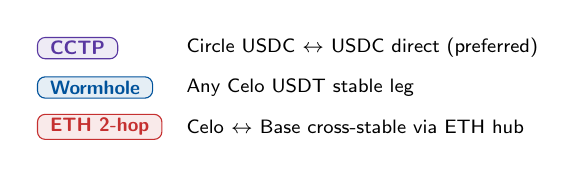
\begin{tikzpicture}[x=1mm,y=1mm,baseline=(a.base)]
\node[anchor=west](a) at(0,0.0){\bridgebadge{CCTP}{routeb}};\node[anchor=west,font=\fontsize{6.6}{8}\selectfont]at(19,0.0){Circle USDC $\leftrightarrow$ USDC direct (preferred)};
\node[anchor=west] at(0,-5.0){\bridgebadge{Wormhole}{primary}};\node[anchor=west,font=\fontsize{6.6}{8}\selectfont]at(19,-5.0){Any Celo USDT stable leg};
\node[anchor=west] at(0,-10.0){\bridgebadge{ETH 2-hop}{warnstroke}};\node[anchor=west,font=\fontsize{6.6}{8}\selectfont]at(19,-10.0){Celo $\leftrightarrow$ Base cross-stable via ETH hub};
\end{tikzpicture}
\end{minipage}
\vfill
{\fontsize{6.4}{7.8}\selectfont\textcolor{ink!55}{Same asset in / same asset out · bot never opens inventory · buy-backs only close loops · live execution gated by \texttt{ENABLE\_LOOP\_PIPELINE} + \texttt{ENABLE\_LOOP\_EXECUTOR}.}}
\end{document}